\part{Electronic Flight Instruments}

% ==============================================================================
\chapter{Head Down Displays (HDD)}
\label{chap:hdd}

Readouts are color coded. Information will be presented in white when in the normal operating range, yellow for information out of the normal range but not out of limits, and red for out of limit values.

PFD Data Presentation: Coloring is used to further segregate differing sources of information. Cyan denotes Pilots input reference set, Amber denotes Flight director.

\newpage
\section{Primary Flight Display (PFD)}
\label{sec:pfd}

The \gls{PFD}, \gls{HSI}, ...

\begin{figure}[h]
  \centering
  \colorbox{black}{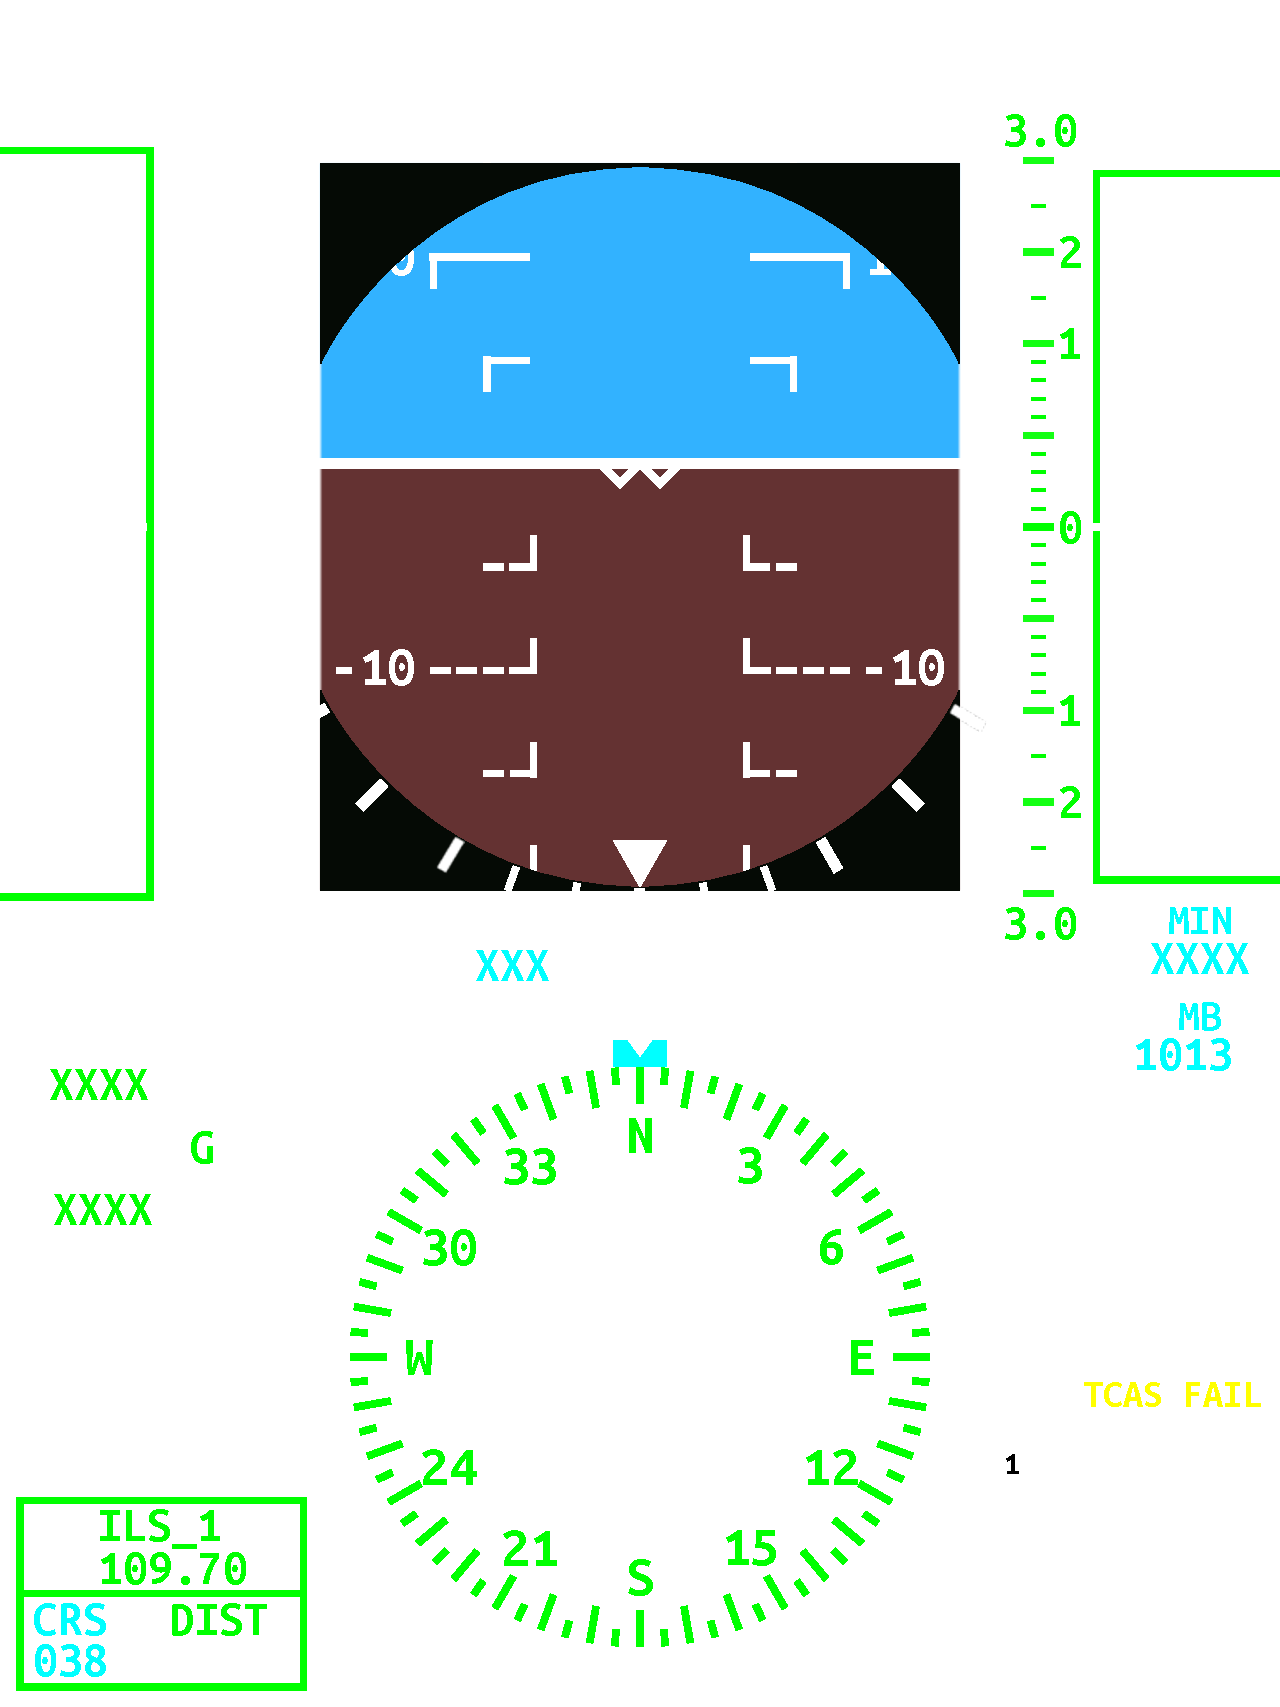
\includegraphics[width=7cm]{figures/hdd/PFD}}
  \caption{Primary Flight Display}
\end{figure}

cyan for VOR/ILS, magenta for FMS

Entered V1 and VR will automatically display on the airspeed indication.

\subsection{Horizontal Situation Indicator (HSI)}
\label{sec:hsi}

Displays Heading, Track, \gls{CDI}, Heading Bug (cyan), Bearing pointers (VOR green, ADF cyan)

\paragraph*{V Speeds}

\begin{itemize}
  \itembf{$V_1$} Critical engine failure recognition speed.
  \itembf{$V_R$} Rotation speed.
  \itembf{$V_{OBS}$} Obstacle clearance speed.
  \itembf{$V_{FUSS}$} Flaps Up Safety Speed.
  \itembf{$V_H$} Maximum speed in level flight at maximum continuous power. (recommended clean max. speed)
\end{itemize}

\paragraph*{Autopilot}

\begin{itemize}
  \item left-top (green): HDG, NAV CAPT, (BACK LOC)?
  \item left-bottom (white): NAV ARM

  \item right-top (green): ALT HOLD, GO ARND, GS CAPT, (CAT2)?
  \item right-bottom (white): ALT SEL, GS ARM, (CAT2 ARM)?
\end{itemize}

For coupled autopilot operation the altitude hold mode is automatically disengaged when:

\begin{itemize}
\item The elevator trim switch or pitch wheel is activated
\item When Vertical Speed (VS), pitch synchronization (SYN), or airspeed (IAS) mode is engaged
\item At glide slope capture in the APPR mode
\end{itemize}

At one thousand feet prior to the selected altitude (ascending or descending) a voice message of A THOUSAND TO GO will alert the crew to approaching altitude selection.

Inflight, the reference IAS cannot be set below 1.2 Vs. With weight on wheels, the reference airspeed is fixed to V2.

In the Primary Flight Display or Heads-Up Display, when either autopilot is engaged (pitch and roll axis), the shape of both Climb Dive Markers (CDM) change from a circle to a diamond.

\newpage
\section{Engine}

\begin{figure}[h]
  \centering
  \colorbox{black}{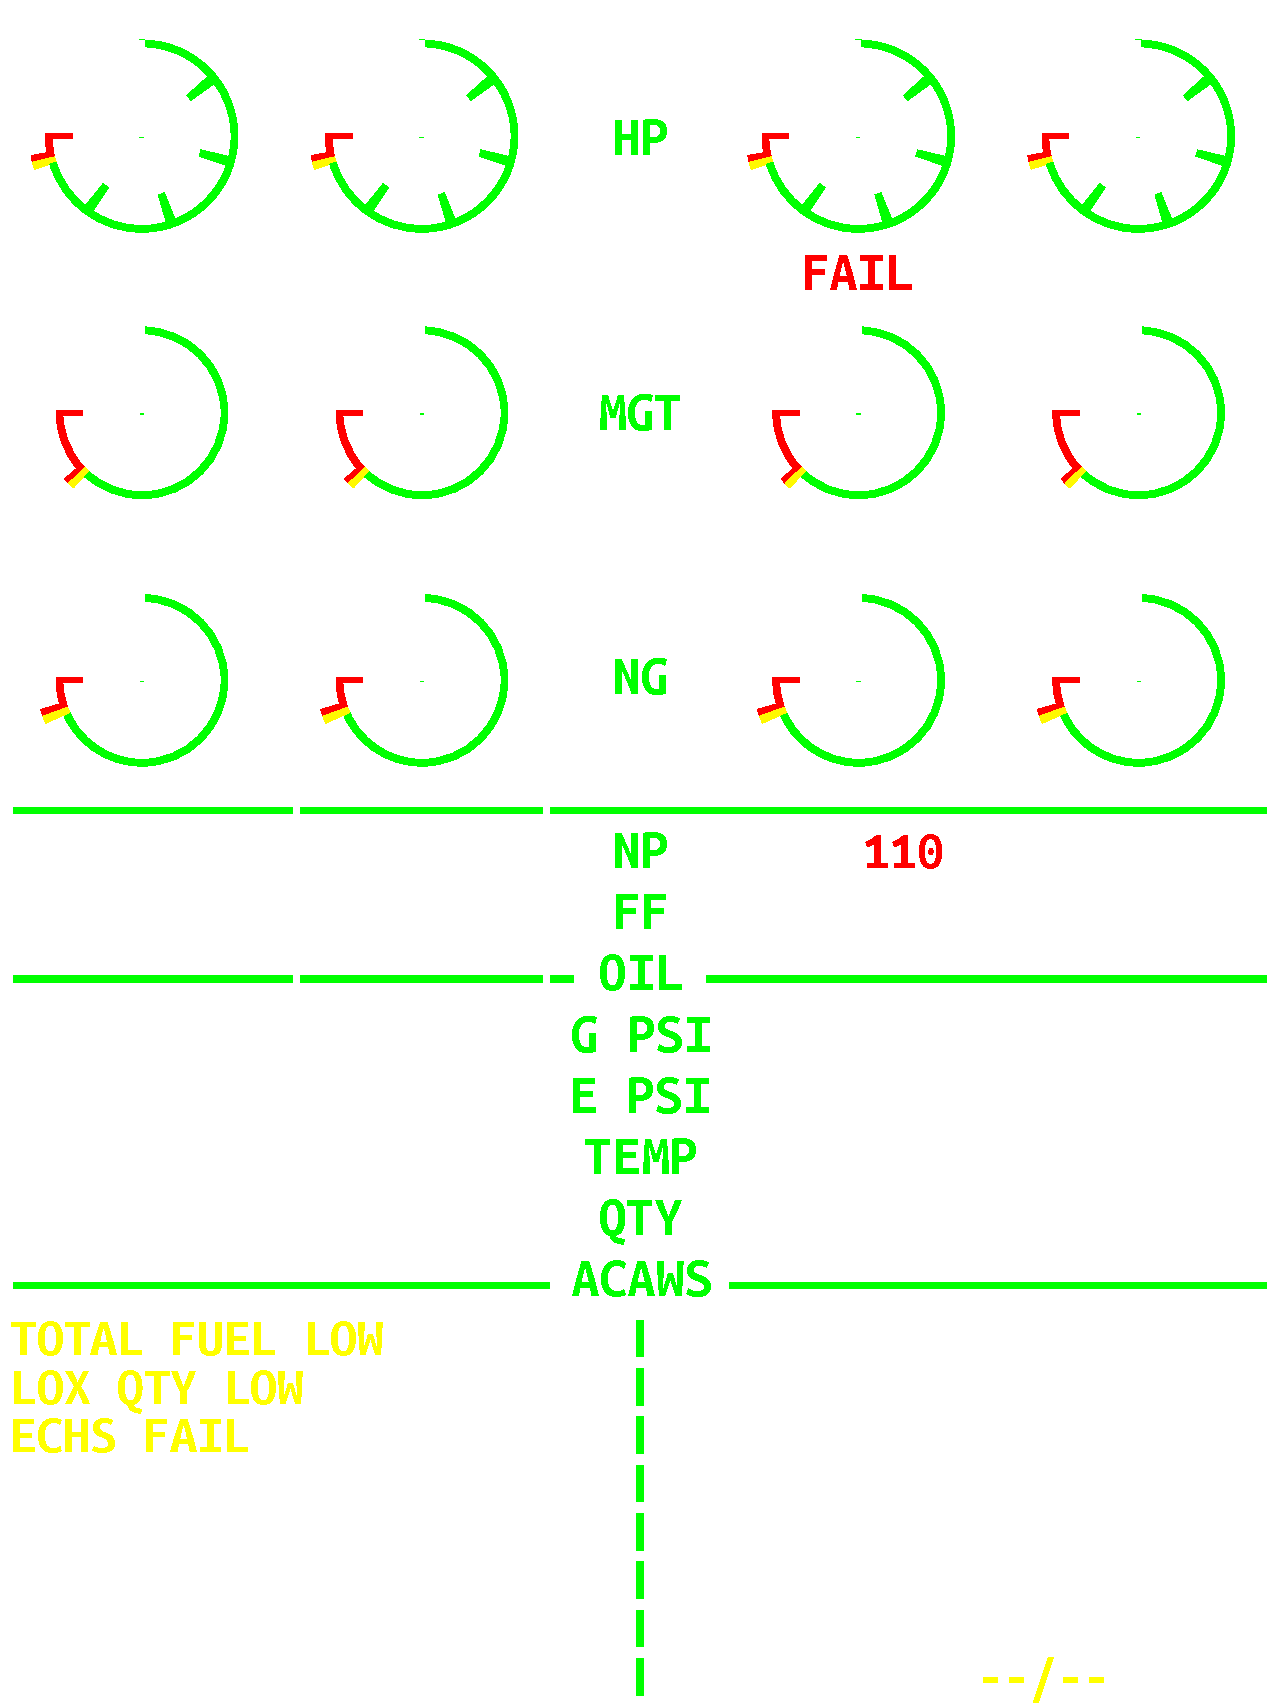
\includegraphics[width=7cm]{figures/hdd/EICAS}}
  \caption{ENGINE and ACAWS display}
\end{figure}

\newpage
\section{CAPS}
\label{sec:caps-airdrop}

\gls{CAPS-airdrop}

\begin{figure}[h]
  \centering
  \colorbox{black}{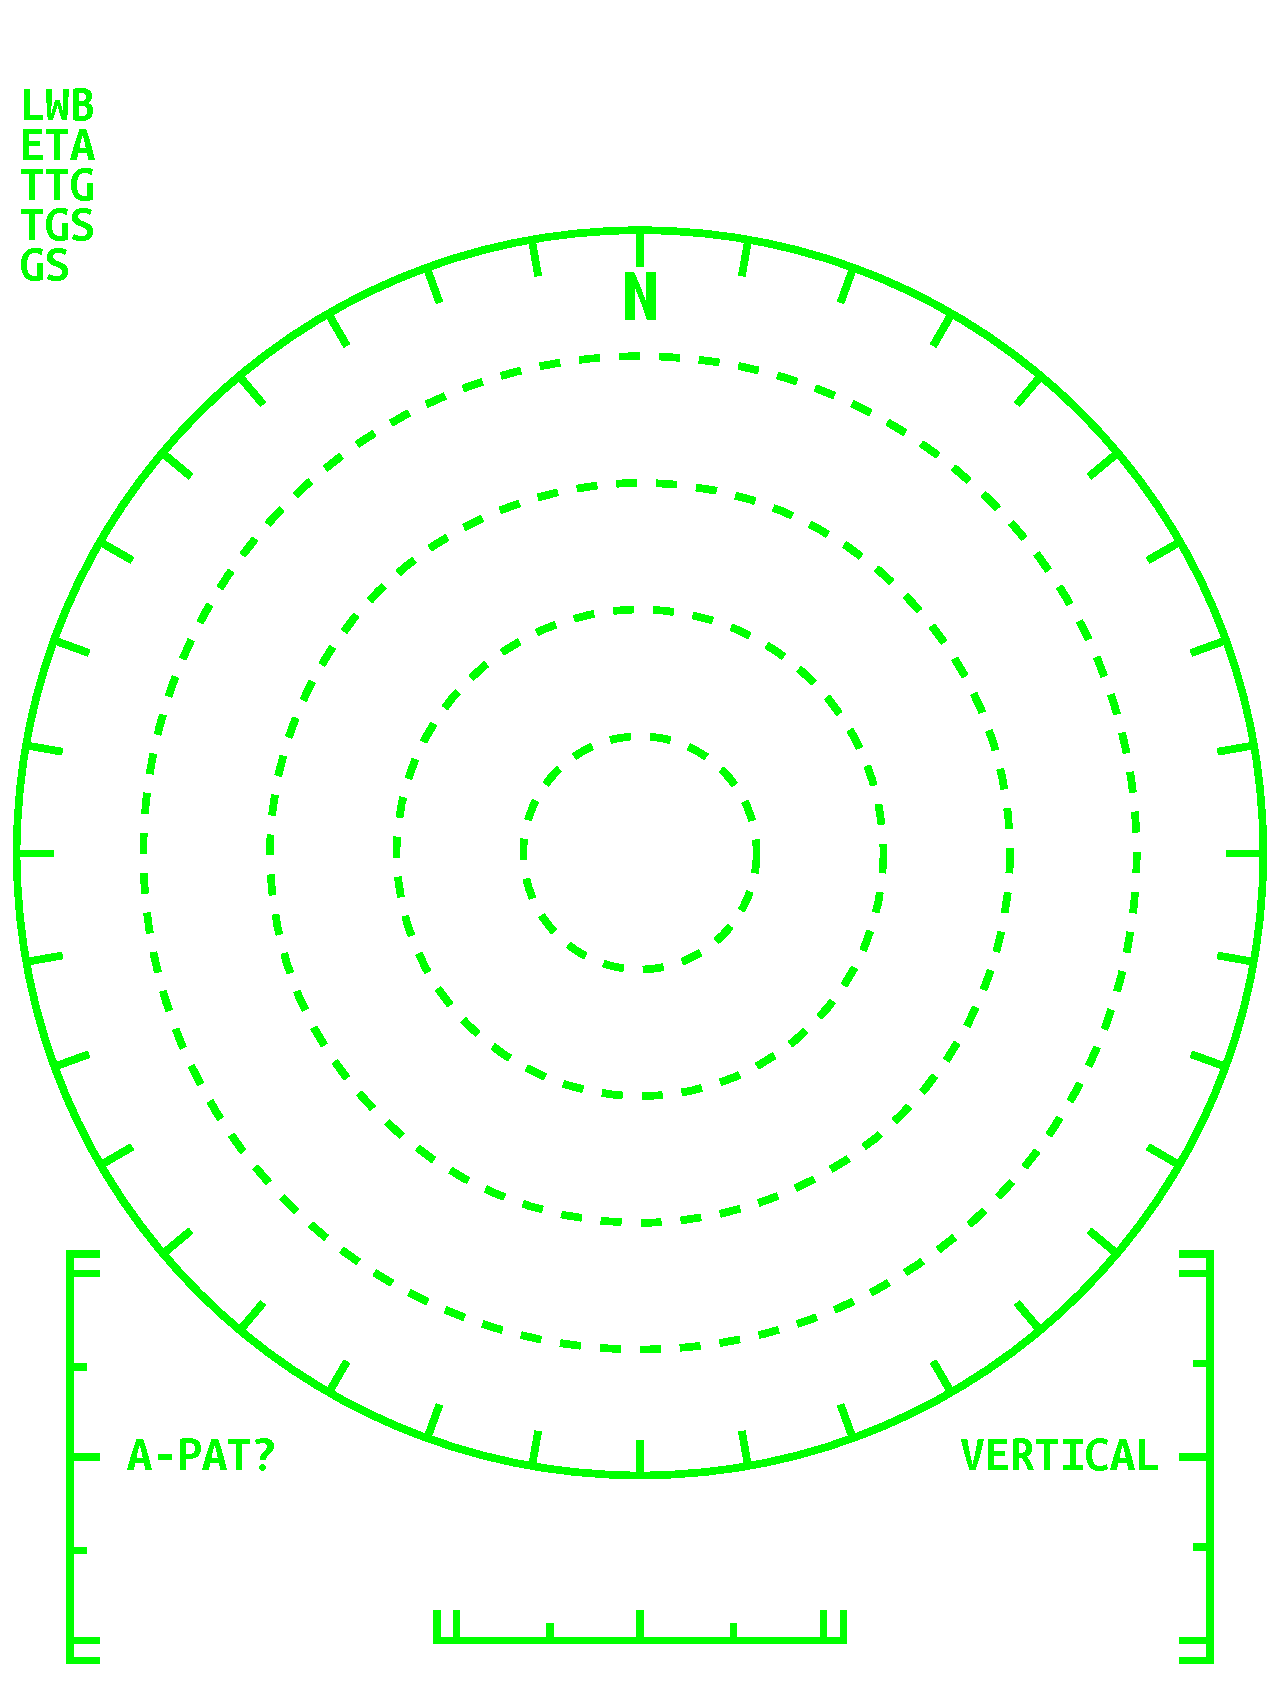
\includegraphics[width=7cm]{figures/hdd/CAPS}}
  \caption{\gls{CAPS-airdrop} display}
\end{figure}

\newpage
\section{System Status}

The SYSTEM STATUS display consists of multiple sections:

\begin{figure}[h]
  \centering
  \colorbox{black}{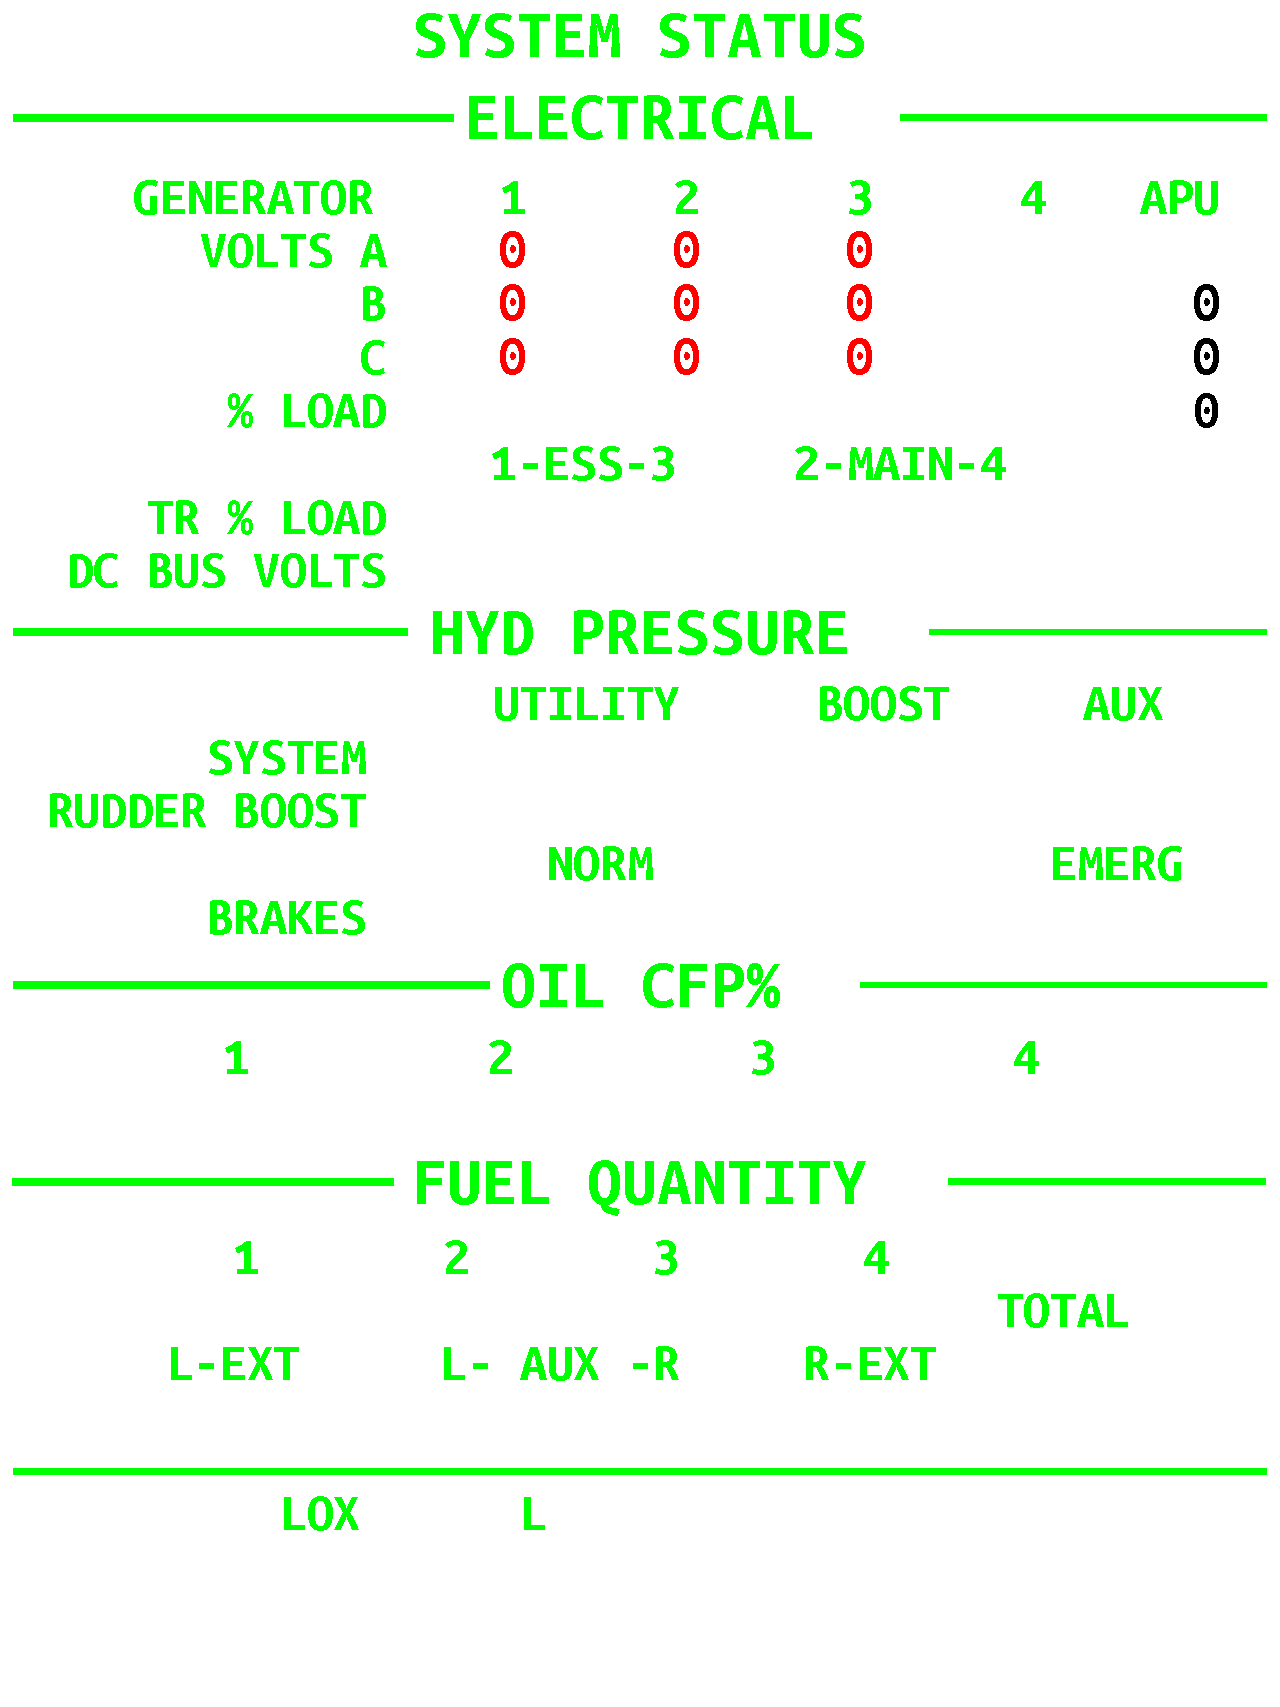
\includegraphics[width=7cm]{figures/hdd/SYSTEM-STATUS}}
  \caption{SYSTEM STATUS display}
\end{figure}

\subsection*{ELECTRICAL}
Generator voltage and percentage of rated current load are shown. Values for generator voltage and load are displayed in columns, labeled from left to right, representing generators 1, 2, 3, 4 and the APU generator. Three voltages are shown in the column for each generator to indicate the voltage of each of the three phases of the generator: A phase, B phase, C phase. Percent of maximum rated load for all five generators (an average of the three phases) is displayed in the row below the C phase voltage. If the system is not powered, OFF will be displayed in the appropriate data blocks. If the system is disconnected (eg. EXT PWR/OFF/APU not APU for APU), three dashed lines will be displayed. The display symbols are generated by the multifunction display units based on information received from the mission computer. 

\subsection*{HYD PRESSURE}

\subsection*{OIL CFP\%}

\subsection*{FUEL QUANTITY}

% ==============================================================================
\chapter{AMU}
\label{chap:amu}

The \gls{AMU}, \gls{CNBP}, \gls{CMDU}, \gls{CMDS}, \gls{CADC}

The CNBP page accesses three scratch pads in the following order: The CNBP, the copilot's CNI-MU and the pilot's CNI-MU. (Ref: T.O. 1C-130(M)J-1 Pg: 2D-66 Chap: 2D)

% ==============================================================================
\chapter{Misc}

\section{LPCR}

\begin{itemize}
\item Weather (WX) Mode of the LPCR: Excessive precipitation (>50 mm/hr) is depicted as magenta on the LPCR display when WX mode is selected.
\item Turbulence is depicted as white in the weather radar mode.
\item Wind shear hazard is processed and displayed for up to 5NM of range coverage.
\item LPCR: The weather mode includes an auto-tilt feature to reduce pilot workload. During auto-tilt, the radar automatically calculates an antenna tilt position that allows the radar beam to remain just above the terrain  at a distance equal to the selected range scale.
\item AUTONAV causes an automatic gyrocompass  alignment and requires only a one-button push to align the EGIs, select all available sensors, and choose the best navigation source by setting the AUTO/MAN LSK to AUTO.
\item Pressing the AUTONAV on the power up page initiates: INU GC alignment, align EGIs, selects all available navigation sensors, navigation source set to (MANUAL)?
\item The FROM/TO page allows for entry of two reference points and a selected groundspeed, and computes the bearing, distance, and time between the two points. To find bearing distance from your present position to the Davis-Monthan AFB TACAN, enter /DMA or PPOS/DMA.
\item The HUD display modes are basic and visual. Basic is the default mode. Visual eliminates the airspeed, altitude, bank, and heading scales, leaving only digital readouts.
\end{itemize}
